\documentclass{standalone}
\usepackage{tikz}
\usetikzlibrary{patterns, positioning}


\begin{document}
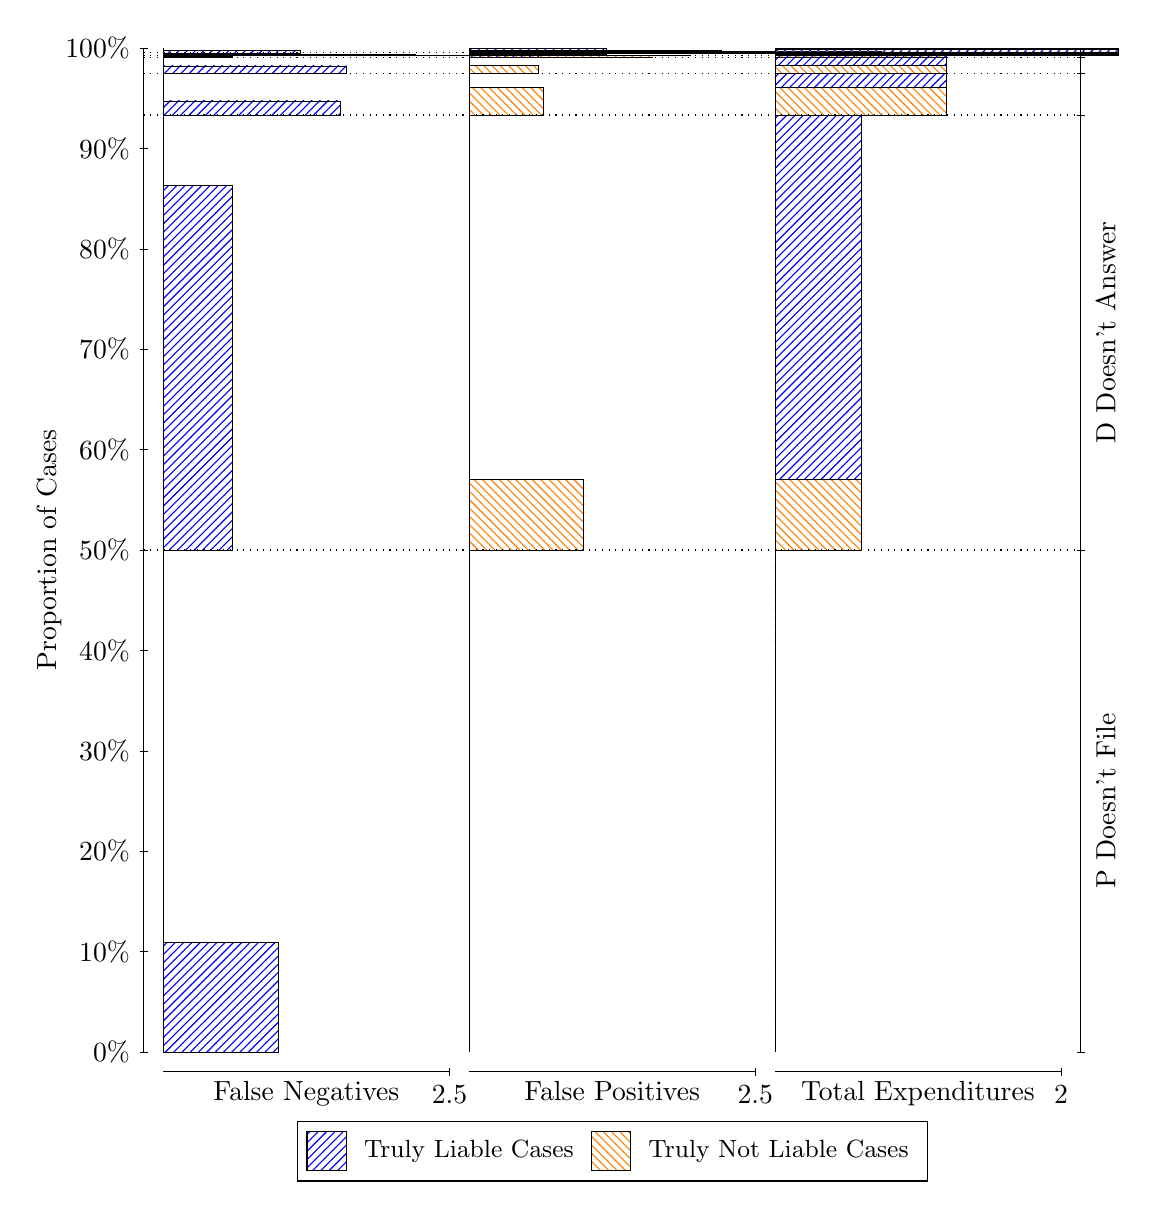
\begin{tikzpicture}
\draw[black, very thin] (1.5,1.75) -- (1.5,14.5);
\node[rotate=90, text=black, anchor=center] at (0.3, 8.125) {Proportion of Cases};
\draw[black, very thin] (1.45,1.75) -- (1.55,1.75);
\node[text=black, anchor=east] at (1.45, 1.75) {0\%};
\draw[black, very thin] (1.45,3.025) -- (1.55,3.025);
\node[text=black, anchor=east] at (1.45, 3.025) {10\%};
\draw[black, very thin] (1.45,4.3) -- (1.55,4.3);
\node[text=black, anchor=east] at (1.45, 4.3) {20\%};
\draw[black, very thin] (1.45,5.575) -- (1.55,5.575);
\node[text=black, anchor=east] at (1.45, 5.575) {30\%};
\draw[black, very thin] (1.45,6.85) -- (1.55,6.85);
\node[text=black, anchor=east] at (1.45, 6.85) {40\%};
\draw[black, very thin] (1.45,8.125) -- (1.55,8.125);
\node[text=black, anchor=east] at (1.45, 8.125) {50\%};
\draw[black, very thin] (1.45,9.4) -- (1.55,9.4);
\node[text=black, anchor=east] at (1.45, 9.4) {60\%};
\draw[black, very thin] (1.45,10.675) -- (1.55,10.675);
\node[text=black, anchor=east] at (1.45, 10.675) {70\%};
\draw[black, very thin] (1.45,11.95) -- (1.55,11.95);
\node[text=black, anchor=east] at (1.45, 11.95) {80\%};
\draw[black, very thin] (1.45,13.225) -- (1.55,13.225);
\node[text=black, anchor=east] at (1.45, 13.225) {90\%};
\draw[black, very thin] (1.45,14.5) -- (1.55,14.5);
\node[text=black, anchor=east] at (1.45, 14.5) {100\%};

\draw[black, very thin] (13.4,1.75) -- (13.4,14.5);
\draw[black, very thin] (13.35,1.75) -- (13.45,1.75);
\node[anchor=west] at (13.35, 1.75) {};
\draw[black, very thin] (13.35,8.1251) -- (13.45,8.1251);
\node[anchor=west] at (13.35, 8.1251) {};
\draw[black, very thin] (13.35,13.649) -- (13.45,13.649);
\node[anchor=west] at (13.35, 13.649) {};
\draw[black, very thin] (13.35,14.178) -- (13.45,14.178);
\node[anchor=west] at (13.35, 14.178) {};
\draw[black, very thin] (13.35,14.379) -- (13.45,14.379);
\node[anchor=west] at (13.35, 14.379) {};
\draw[black, very thin] (13.35,14.405) -- (13.45,14.405);
\node[anchor=west] at (13.35, 14.405) {};
\draw[black, very thin] (13.35,14.438) -- (13.45,14.438);
\node[anchor=west] at (13.35, 14.438) {};
\draw[black, very thin] (13.35,14.5) -- (13.45,14.5);
\node[anchor=west] at (13.35, 14.5) {};

\draw[black, very thin, pattern color=blue, pattern=north east lines] (1.75,1.75) rectangle (3.2033,3.1452);
\draw[black, very thin, pattern color=orange, pattern=north west lines] (1.75,3.1452) rectangle (1.75,8.1251);
\draw[black, very thin, pattern color=blue, pattern=north east lines] (1.75,8.1251) rectangle (2.622,12.751);
\draw[black, very thin, pattern color=orange, pattern=north west lines] (1.75,12.751) rectangle (1.75,13.649);
\draw[black, very thin, pattern color=blue, pattern=north east lines] (1.75,13.649) rectangle (4.0027,13.828);
\draw[black, very thin, pattern color=orange, pattern=north west lines] (1.75,13.828) rectangle (1.75,14.178);
\draw[black, very thin, pattern color=blue, pattern=north east lines] (1.75,14.178) rectangle (4.0753,14.273);
\draw[black, very thin, pattern color=orange, pattern=north west lines] (1.75,14.273) rectangle (1.75,14.379);
\draw[black, very thin, pattern color=blue, pattern=north east lines] (1.75,14.379) rectangle (2.622,14.396);
\draw[black, very thin, pattern color=orange, pattern=north west lines] (1.75,14.396) rectangle (1.75,14.405);
\draw[black, very thin, pattern color=blue, pattern=north east lines] (1.75,14.405) rectangle (8.4353,14.407);
\draw[black, very thin, pattern color=blue, pattern=north east lines] (1.75,14.407) rectangle (4.9473,14.421);
\draw[black, very thin, pattern color=orange, pattern=north west lines] (1.75,14.421) rectangle (1.75,14.438);
\draw[black, very thin, pattern color=blue, pattern=north east lines] (1.75,14.438) rectangle (3.494,14.469);
\draw[black, very thin, pattern color=orange, pattern=north west lines] (1.75,14.469) rectangle (1.75,14.485);
\draw[black, very thin, pattern color=blue, pattern=north east lines] (1.75,14.485) rectangle (1.75,14.5);
\draw[black, very thin, pattern color=orange, pattern=north west lines] (5.6333,1.75) rectangle (5.6333,6.73);
\draw[black, very thin, pattern color=blue, pattern=north east lines] (5.6333,6.73) rectangle (5.6333,8.1251);
\draw[black, very thin, pattern color=orange, pattern=north west lines] (5.6333,8.1251) rectangle (7.0867,9.0233);
\draw[black, very thin, pattern color=blue, pattern=north east lines] (5.6333,9.0233) rectangle (5.6333,13.649);
\draw[black, very thin, pattern color=orange, pattern=north west lines] (5.6333,13.649) rectangle (6.578,13.999);
\draw[black, very thin, pattern color=blue, pattern=north east lines] (5.6333,13.999) rectangle (5.6333,14.178);
\draw[black, very thin, pattern color=orange, pattern=north west lines] (5.6333,14.178) rectangle (6.5053,14.283);
\draw[black, very thin, pattern color=blue, pattern=north east lines] (5.6333,14.283) rectangle (5.6333,14.379);
\draw[black, very thin, pattern color=orange, pattern=north west lines] (5.6333,14.379) rectangle (7.9587,14.388);
\draw[black, very thin, pattern color=blue, pattern=north east lines] (5.6333,14.388) rectangle (6.5053,14.405);
\draw[black, very thin, pattern color=orange, pattern=north west lines] (5.6333,14.405) rectangle (7.3773,14.419);
\draw[black, very thin, pattern color=blue, pattern=north east lines] (5.6333,14.419) rectangle (5.924,14.433);
\draw[black, very thin, pattern color=orange, pattern=north west lines] (5.6333,14.433) rectangle (5.6333,14.436);
\draw[black, very thin, pattern color=blue, pattern=north east lines] (5.6333,14.436) rectangle (5.6333,14.438);
\draw[black, very thin, pattern color=orange, pattern=north west lines] (5.6333,14.438) rectangle (12.319,14.441);
\draw[black, very thin, pattern color=blue, pattern=north east lines] (5.6333,14.441) rectangle (10.865,14.457);
\draw[black, very thin, pattern color=orange, pattern=north west lines] (5.6333,14.457) rectangle (8.8307,14.469);
\draw[black, very thin, pattern color=blue, pattern=north east lines] (5.6333,14.469) rectangle (7.3773,14.5);
\draw[black, very thin, pattern color=orange, pattern=north west lines] (9.5167,1.75) rectangle (9.5167,6.73);
\draw[black, very thin, pattern color=blue, pattern=north east lines] (9.5167,6.73) rectangle (9.5167,8.1251);
\draw[black, very thin, pattern color=orange, pattern=north west lines] (9.5167,8.1251) rectangle (10.607,9.0233);
\draw[black, very thin, pattern color=blue, pattern=north east lines] (9.5167,9.0233) rectangle (10.607,13.649);
\draw[black, very thin, pattern color=orange, pattern=north west lines] (9.5167,13.649) rectangle (11.697,13.999);
\draw[black, very thin, pattern color=blue, pattern=north east lines] (9.5167,13.999) rectangle (11.697,14.178);
\draw[black, very thin, pattern color=orange, pattern=north west lines] (9.5167,14.178) rectangle (11.697,14.283);
\draw[black, very thin, pattern color=blue, pattern=north east lines] (9.5167,14.283) rectangle (11.697,14.379);
\draw[black, very thin, pattern color=orange, pattern=north west lines] (9.5167,14.379) rectangle (11.697,14.388);
\draw[black, very thin, pattern color=blue, pattern=north east lines] (9.5167,14.388) rectangle (11.697,14.405);
\draw[black, very thin, pattern color=orange, pattern=north west lines] (9.5167,14.405) rectangle (13.877,14.419);
\draw[black, very thin, pattern color=blue, pattern=north east lines] (9.5167,14.419) rectangle (13.877,14.433);
\draw[black, very thin, pattern color=orange, pattern=north west lines] (9.5167,14.433) rectangle (13.877,14.436);
\draw[black, very thin, pattern color=blue, pattern=north east lines] (9.5167,14.436) rectangle (13.877,14.438);
\draw[black, very thin, pattern color=orange, pattern=north west lines] (9.5167,14.438) rectangle (13.877,14.451);
\draw[black, very thin, pattern color=blue, pattern=north east lines] (9.5167,14.451) rectangle (13.877,14.482);
\draw[black, very thin, pattern color=orange, pattern=north west lines] (9.5167,14.482) rectangle (13.877,14.485);
\draw[black, very thin, pattern color=blue, pattern=north east lines] (9.5167,14.485) rectangle (13.877,14.5);
\draw[black, dotted] (1.5,8.1251) -- (13.4,8.1251);
\draw[black, dotted] (1.5,13.649) -- (13.4,13.649);
\draw[black, dotted] (1.5,14.178) -- (13.4,14.178);
\draw[black, dotted] (1.5,14.379) -- (13.4,14.379);
\draw[black, dotted] (1.5,14.405) -- (13.4,14.405);
\draw[black, dotted] (1.5,14.438) -- (13.4,14.438);
\draw[black, very thin] (1.75,1.5) -- (5.3833,1.5);
\node[text=black, anchor=north] at (3.5667, 1.5) {False Negatives};
\draw[black, very thin] (5.3833,1.45) -- (5.3833,1.55);
\node[text=black, anchor=north] at (5.3833, 1.45) {2.5};

\draw[black, very thin] (5.6333,1.5) -- (9.2667,1.5);
\node[text=black, anchor=north] at (7.45, 1.5) {False Positives};
\draw[black, very thin] (9.2667,1.45) -- (9.2667,1.55);
\node[text=black, anchor=north] at (9.2667, 1.45) {2.5};

\draw[black, very thin] (9.5167,1.5) -- (13.15,1.5);
\node[text=black, anchor=north] at (11.333, 1.5) {Total Expenditures};
\draw[black, very thin] (13.15,1.45) -- (13.15,1.55);
\node[text=black, anchor=north] at (13.15, 1.45) {2};

\node[text=black, centered, rotate=90] at (13.72, 4.9376) {P Doesn't File};
\node[text=black, centered, rotate=90] at (13.72, 10.887) {D Doesn't Answer};






\draw (7.449999999999999,1.5) node[draw=none] (baseCoordinate) {};
\begin{scope}[align=center]
        \matrix[scale=0.5, draw=black, below=0.5cm of baseCoordinate, nodes={draw}, column sep=0.1cm]{
            \node[rectangle, draw, minimum width=0.5cm, minimum height=0.5cm, pattern color=blue, pattern=north east lines] {}; &
            \node[draw=none, font=\small, text=black] (B) {Truly Liable Cases}; &
            \node[rectangle, draw, minimum width=0.5cm, minimum height=0.5cm, pattern color=orange, pattern=north west lines] {}; &
            \node[draw=none, font=\small, text=black] (B) {Truly Not Liable Cases}; \\
            };
\end{scope}

\end{tikzpicture}
\end{document}